\begin{frame}{RCPSP and CECSP}
interet modele a evenemtn

partie commune des modele

c'est sur ça qu'on travaille

a quoi ça correspond
\end{frame}
  \subsubsection{Valid inequalities}

\begin{frame}
  \frametitle{Maximum separation between events}
  \begin{itemize}
  \item {\bf Goal: } upper bound on the value of $t_{e+1}-t_{e}$
    \vspace{0.3cm}
  \item<2-> time window of each task start and/or end time
    \vspace{0.3cm}
  \item<8-> an event must occur in each of these time windows
    \vspace{0.3cm}
  \item<13-> two consecutive events in the union of two consecutive time windows
  \end{itemize}
  \vfill
  \onslide<3->{
    \begin{center} 
      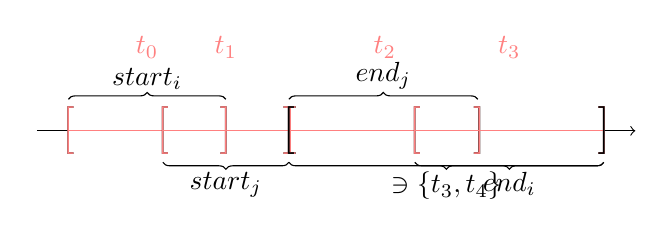
\begin{tikzpicture}
        [decoration={brace},scale=0.4]
        \node (O) at (0,0) {}; 
        
        \draw[->] (0,0) -- (19,0);
        \onslide<4-12>{
          \path (1,0) node {\LARGE [} -- +(0:5cm)node {\LARGE ]};
          \onslide<9>{
            \path[red!50,draw] (1,0) node {\LARGE [} -- +(0:5cm)node
            {\LARGE ]} node[midway,above=0.8cm] {$t_0$};
          }
          \onslide<4>{
            \draw [decorate] (1,1) -- +(0:5cm) node[midway,above]
            {$start_i$};
          }
          \path(4,0) node {\LARGE [} -- +(0:4cm) node {\LARGE ]} ;
        \onslide<10>{
          \path[red!50,draw](4,0) node {\LARGE [} -- +(0:4cm) node {\LARGE ]} node[midway,above=0.8cm] {$t_1$};
        } 
        \onslide<5>{\draw [decorate] (8,-1) -- +(0:-4cm) node[midway,below]
          {$start_j$};
        }
      }
      \onslide<4-13>{
        \onslide<10>{\path (8.05,0) node {}  --
          +(0:6cm) node {\LARGE ]}  ;}
        \onslide<11-13>{\path (8.05,0) node {\LARGE [}  --
          +(0:6cm) node {\LARGE ]}  ;}
       \onslide<4-9>{\path (8.05,0) node {\LARGE [}  --
          +(0:6cm) node {\LARGE ]}  ;}
        \onslide<11>{
          \path[red!50,draw] (8.05,0) node {\LARGE [}  --
          +(0:6cm) node {\LARGE ]}  node[midway,above=0.8cm] {$t_2$};
        }
        \onslide<6>{ 
          \draw [decorate] (8,1) -- +(0:6cm) node[midway,above]
          {$end_j$};
        }

        \path (12,0) node {\LARGE [} --
        +(0:6cm) node {\LARGE ]} ;
        \onslide<12>{
          \path[red!50,draw] (12,0) node {\LARGE [} --
          +(0:6cm) node {\LARGE ]} node[midway,above=0.8cm] {$t_3$};
        }    
        \onslide<7>{\draw [decorate] (18,-1) -- +(0:-6cm)
          node[midway,below] {$end_i$};
        }
      }
      \onslide<14>{
        \path (8,0) node {\LARGE [} --
        +(0:10cm) node {\LARGE ]}  ;
        \draw [decorate] (18,-1) -- +(0:-10cm)
        node[midway,below] {$\ni \{t_3,t_{4}\}$};
      }
    \end{tikzpicture}
  \end{center}
}
\end{frame}

\begin{frame}
  \frametitle{Maximum separation between events}
  \begin{itemize}
  \item Order the time-window intervals according to:
    \[ [{\cal S}_x^1,{\cal S}_y^1] \le [{\cal S}_x^2,{\cal S}_y^2]
      \Leftrightarrow 	{\cal S}_x^1 < {\cal S}_x^2 \lor \left( {\cal
          S}_x^1={\cal S}_x^2 \land {\cal S}_y^1\le {\cal
          S}_y^2\right)\]
\vfill
  \item Then we have:
\[t_{e+1}-t_e \le  
|{\cal S}_e \cup {\cal S}_{e+1}| 
\]
\vfill
  \item We can use it as:
\begin{itemize}
\vspace{0.2cm}
\item additional constraints of the model
\item in $ b_{ie} \ge \bmin(t_{e+1}-t_e) -  (\bmin(d_i-r_i)(1-z_{i,e})
  )$ instead of $d_i-r_i$
\end{itemize}
  \end{itemize}
\end{frame}

\begin{frame}
  \frametitle{Maximum time for an event}
  \begin{itemize}
  \item {\bf Goal: } upper bound on the value of $t_{e}$
    \vspace{0.4cm}
  \item<2-> upper bound of each task start and/or end time
    \vspace{0.4cm}
  \item<5-> an event must occur before each of these upper bound
    \vspace{0.4cm}
  \end{itemize}
  \vfill
  \onslide<3->{
    \begin{center} 
      \begin{tikzpicture}
        [decoration={brace},scale=0.4]
        \node (O) at (0,0) {}; 
        
        \draw[->] (0,0) -- (19,0);
        \onslide<3>{
          \draw (1,0) node {\LARGE [} -- +(0:5cm)node {\LARGE ]}; 
        
        \draw(4,0) node {\LARGE [} -- +(0:4cm) node {\LARGE ]} ;
   
        \draw (8.05,0) node {\LARGE [}  --
        +(0:6cm) node {\LARGE ]}  ;
                \draw (12,0) node {\LARGE [} --
        +(0:6cm) node {\LARGE ]}  ;}
      \onslide<4>{
  
        \draw (1,0) node {} -- +(0:5cm)node {\LARGE ]}; 
        
        \draw(4,0) node {} -- +(0:4cm) node {\LARGE ]} ;
   
        \draw (8.05,0) node {}  --
        +(0:6cm) node {\LARGE ]}  ;
                \draw (12,0) node {} --
        +(0:6cm) node {\LARGE ]}  ;}
      \onslide<5>{
          \draw[color=red!50] (0,0) node {} -- +(0:6cm)node {\LARGE ]}
          node[left,above=0.8cm] {$t_0$}; 
          \draw (8,0) node {\LARGE ]} ;
          \draw (8.05,0) node {}  -- +(0:6cm) node {\LARGE ]}  ;
          \draw (12,0) node {} -- +(0:6cm) node {\LARGE ]}  ;}
      
        \onslide<6>{
          \draw (6,0) node  {\LARGE ]}; 
          \draw[color=red!50](0,0) -- (8,0) node {\LARGE ]} node[left,above=0.8cm] {$t_1$};
          \draw (8.05,0) node {}  --  +(0:6cm) node {\LARGE ]}  ;
          \draw (12,0) node {} --  +(0:6cm) node {\LARGE ]}  ;}
      
        \onslide<7>{
          \draw (6,0) node {\LARGE ]}; 
          \draw (8,0) node {\LARGE ]} ;
          \draw[color=red!50] (0,0) node {}  -- (14,0) node {\LARGE ]} node[left,above=0.8cm] {$t_2$} ;
          \draw (18,0)node {\LARGE ]}  ;}
        
        \onslide<8>{
          \draw (6,0) node {\LARGE ]}; 
          \draw(8,0) node {\LARGE ]} ;
          \draw (14,0) node {\LARGE ]}  ;
          \draw[color=red!50] (0,0) node {} -- (18,0) node {\LARGE ]}
          node[left,above=0.8cm] {$t_3$};} 
      
      \end{tikzpicture}
    \end{center}
  }
\end{frame}


\begin{frame}
  \frametitle{Maximum time for an event}
  \begin{itemize}
  \item Order the time-window interval upper bounds ${\cal UP}$ in
    increasing order 
\vfill
  \item Then we have:
\[t_e \le  {\cal UP}_e\]
\vfill
\item We can use it as:
\begin{itemize}
  \vspace{0.2cm}
\item additional constraints of the model
\item in $ t_e \le
  s_i^{max}(z_{i,e}-z_{i,e-1})+(1-(z_{i,e}-z_{i,e-1}))T $
  and $ t_e \le d_i(z_{i,e-1}-z_{i,e})+(1-(z_{i,e-1}-z_{i,e}))T$ instead of $T$
\end{itemize}
  \end{itemize}
\end{frame}
\subsubsection{Polyhedral results}
\begin{frame}
  \frametitle{$Z$-polyhedron}
  \vfill
  \begin{overlayarea}{\linewidth}{3.5cm}
    \only<1-3>{
      \begin{itemize}
      \item<1-> defined by the $z_{i,e}$ on/off variable
      \item<2-> for a single activity $i$:
        \[ZQ_i= conv\{z_i \in \{0,1\}^{|{\cal E}|} | z_i \text{ has
            the consecutive-one property}\} \] 
        \onslide<3-3>{
        e.g. $(0,0,1,1,1,0),\ (1,1,1,0,0,0),\ \dots$}
      \end{itemize}
    }
    \only<4->{
      \begin{itemize}
      \item<4-> e.g. \[ z_{i,3} - z_{i,6} + z_{i,11}-z_{i,13} +z_{i,18} \le
          1 \]
        \vspace{0.3cm}
      \item<5-> If $|S|=3$ then $ z_{i,e}-z_{i,f}+z_{i,g} \le 1$ enforce
          $z_{i,f}$ to be $1$ for all $e<f<g$ s.t. $z_{i,e}=z_{i,g}=1$ 
      \end{itemize}
    }
  \end{overlayarea}
  \vfill
  \onslide<4->{
  \begin{block}{Non-preemptive inequalities}
    \[\sum_{e_k \in S} (-1)^kz _{i,e_k} \leq 1\]
    where $S = \{e_0,e_1,\ldots,e_{2\ell}\}$ is a subset of 
    ${\cal E}$ of odd cardinality.
  \end{block}
}
\vfill
\end{frame}

\begin{frame}
  \frametitle{$Z$-polyhedron}
  \[ZP_i=\{ z_i \in [0,1]^{\cal E} | z_i\text{ satisfies
      non-preemptive inequalities and } \eqref{eq1}\}\] 
  \pause
  with 
  \begin{equation}
    \sum_{e \in \cal E} z_{i,e} \ge 1 \quad \forall i \in \cal A  
    \label{eq1}  
  \end{equation}
  \pause
  \begin{block}{Theorem}
    \[ZP_i=ZQ_i\]
  \end{block}
  \vspace{0.3cm}
 \onslide<5->{ {\bf Proof} uses Farkas lemma
  }
  \onslide<4->{\[ZQ_i= conv\{z_i \in \{0,1\}^{|{\cal E}|} | z_i \text{ has the consecutive
      one property}\} \]
}

\end{frame}


\begin{frame}
\frametitle{Computational experience}
\begin{itemize}
\vfill
\item Intel Core i7-4770 processor with 4 cores and 8Go of RAM
\vfill
\item OS: 64-bit Ubuntu 12.04
\vfill
\item MILP resolution: CPLEX 12.6 with 1 thread  
\vfill
\item Special separation procedure for non-preemptive cuts ($O(n^2)$)
  for node with depth less than 10
\vfill
\item time limit: 1000 seconds
\vfill
\end{itemize}
\end{frame}

\begin{frame}
\frametitle{Time comparison for the CECSP}
\begin{itemize}
\item Instance of {\it [Nattaf et al.,2015]}
\item 10 instances of 20, 25 and 30 tasks
\end{itemize}
\vfill
\begin{center}
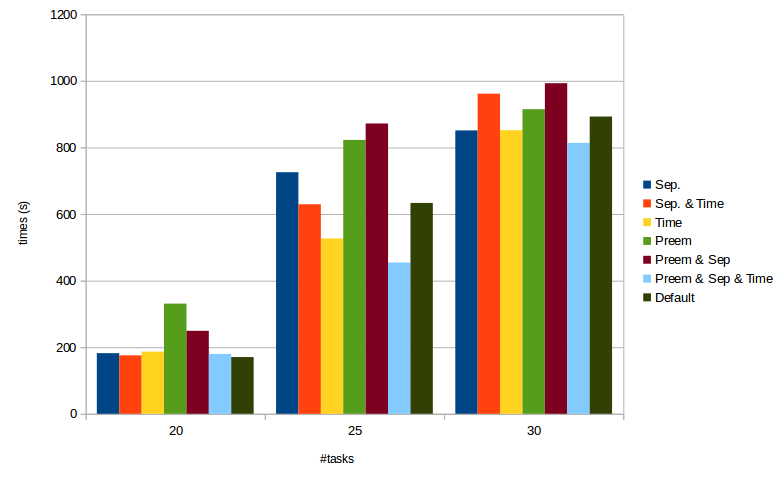
\includegraphics[height=5cm, width=9cm]{time_CECSP.png}
\end{center}
\end{frame}


\begin{frame}
\frametitle{Solved instances comparison for the CECSP}
\begin{itemize}
\item Instance of {\color{gray!50!black!70}\it [Nattaf et al., 2015]}
\item 10 instances of 20, 25 and 30 tasks
\end{itemize}
\vfill
\begin{center}
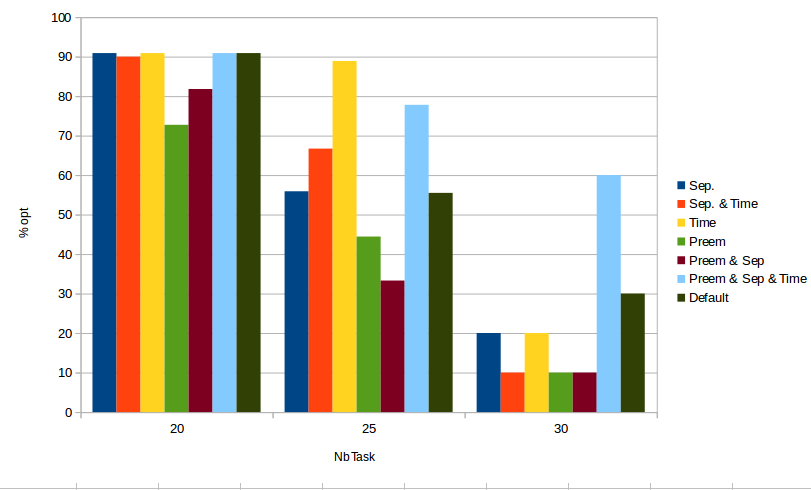
\includegraphics[height=5cm, width=9cm]{opt_CECSP.png}
\end{center}
\end{frame}

\begin{frame}
\frametitle{Time comparison for the RCPSP}
\begin{itemize}
\item Instance of {\color{gray!50!black!70} \it [Koné et al., 2011]}
\item 480 instances of 30 tasks
\end{itemize}
\vfill
\begin{center}
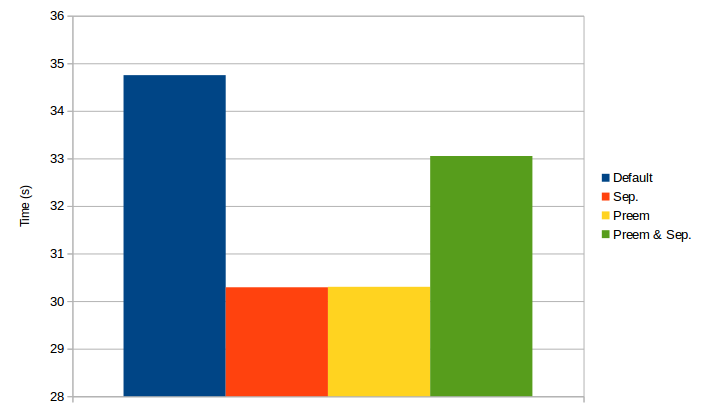
\includegraphics[height=5cm, width=9cm]{timeRCPSP.png}
\end{center}
\end{frame}
